\documentclass[twoside,a4paper,12pt]{book}

\usepackage{polski}
\usepackage[utf8]{inputenc}
\usepackage{amsmath,amssymb,amsthm}
\usepackage{xcolor}
\usepackage[final]{pdfpages}
\usepackage{graphicx}
\usepackage{caption}
\usepackage{subcaption}

\newenvironment{diagrams}[2]{\begin{figure}[!h]
	%\centering
	\begin{subfigure}{.5\textwidth}
		\centering
		\includegraphics[width=.9\textwidth]{#1}
		\caption{}
		\label{#1}
	\end{subfigure}
	\begin{subfigure}{.5\textwidth}
		\centering
		\includegraphics[width=.9\textwidth]{#2}
		\caption{}
		\label{#2}
	\end{subfigure}
	}
	{
	\end{figure}
	}

\begin{document}
	
\begin{titlepage}
	
\includepdf{StronaTytulowa.pdf}
	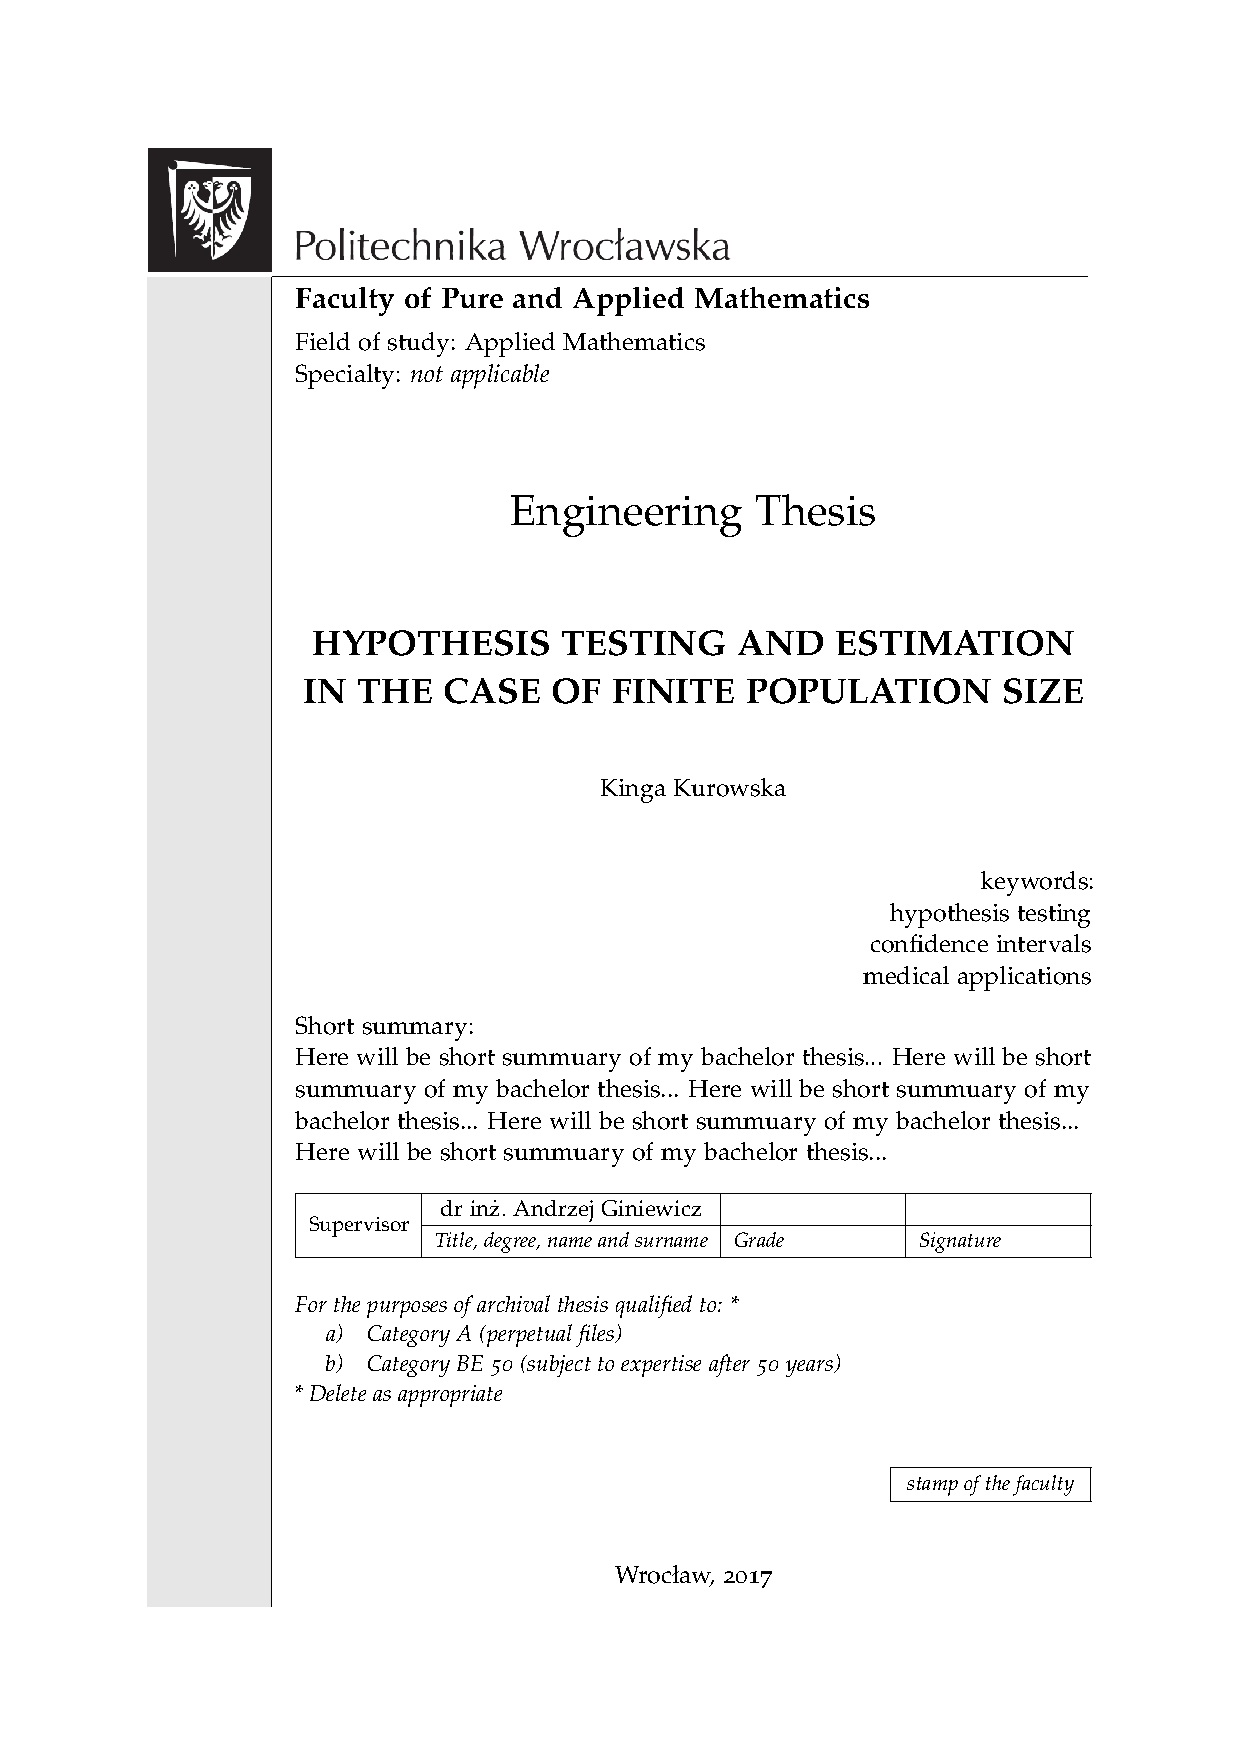
\includepdf{StronaTytulowa_ang.pdf}
\end{titlepage}

\tableofcontents

\chapter*{Wstęp}
Początki teorii rachunku prawdopodobieństwa i~statystyki sięgają XVI~w. Zajmowano się wtedy analizą rzutu kostką oraz prawdopodobieństwem błędów pomiarowych. Już w~XVII wieku Blaise Pascal sformułował i~dowiódł własności trójkąta arytmetycznego oraz użył pojęcia kombinacji~\cite{Hald2003}. Na początku XVIII~wieku opublikowane zostały prace Jacoba Bernoullego, w~których zawarł wiele swoich tez na temat prawdopodobieństwa. Przez te kilka wieków teoria rachunku prawdopodobieństwa i~statystyki znacząco się wzbogaciła i~rozwinęła. Rozpoczęto rozważania na temat estymacji i~testowania hipotez, które są w~naszych czasach zasadniczą domeną statystyki.

W przypadku dyskretnym najczęściej testowane są proporcje populacji~\cite{Lehmann1968}. Chcemy się przekonać czy dana próbka ma jakąś konkretną proporcję albo dwie próbki mają tę samą proporcję elementów z~badaną cechą. Znana jest powszechnie teoria dotycząca testowania hipotez, gdy populacja jest nieskończona, a~raczej na tyle duża, że możemy ją w przybliżeniu uznać za nieskończoną. Wtedy schemat próbkowania jest opisany jako losowanie ze zwracaniem. Jednak przypadek nieskończonej populacji nie wyczerpuje tematu testowania proporcji. Gdy populacja jest bardzo mała albo, gdy próbka jest niewiele mniejsza od całej populacji, schemat próbkowania opiera się o~losowanie bez zwracania. 

Warto zająć się teorią testowania hipotez dla skończonej populacji, ponieważ w~określonych przypadkach testy ze skończoną poprawką dają dużo dokładniejszą informację o~badanym przypadku niż testy zakładające nieskończoną populację. Ponadto zastosowanie tego typu testów ma duże znaczenie w~medycynie, gdzie często rozważane populacje mają na tyle wyspecjalizowane cechy, że są uważane za małe.

W~pierwszym rozdziale znajduje się opis schematu pobierania danych, w~przypadku nieskończonej i~skończonej populacji, oraz porównanie obu sposobów w~oparciu o~własności rozkładów próbek i~estymację przedziałową proporcji. W rozdziale~\ref{r2} przedstawiono testy bez skończonej poprawki oraz z~jej uwzględnieniem. Rozdział~\ref{r3} zawiera porównanie testów na podstawie prawdopodobieństwa błędu I~rodzaju oraz mocy testu. Na końcu pracy znajduje się podsumowanie uzyskanych wyników.
\chapter{Przedstawienie testów}

W tym rozdziale chciałabym opisać dwa testy wykorzystujące rozkład hipergeometryczny oraz test oparty na rozkładzie dwumianowym. Omówię także sposób liczenia prawdopodobieństwa błędu I rodzaju i mocy testu.

\section{Sformułowanie problemu}
Załóżmy, że $X_1$ i $X_2$ są niezależnymi zmiennymi losowymi o rozkładzie hipergeometrycznym $X_1\sim h(n_1,M_1,N_1)$, $X_2\sim h(n_2,M_2,N_2)$. Zaobserwowane wartości $X_1$ i $X_2$ oznaczmy odpowiednio $k_1$ i $k_2$ oraz proporcje $p_1=M_1/N_1$, $p_2=M_2/N_2$. Będę zajmować się testowaniem hipotez
\begin{equation}
H_0{:}\ p_1=p_2\quad \text{przeciwko} \quad H_1{:}\ p_1\neq p_2,
\end{equation}
w oparciu o $(k_1,n_1,N_1)$ i $(k_2,n_2,N_2)$.
Rozważmy unormowaną statystykę
\begin{equation}
Z_{X_1,X_2} = \frac{X_1/n_1-X_2/n_2}{\sqrt{V_{X_1,X_2}}},
\end{equation}
gdzie estymator wariancji pod warunkiem zachodzenia $H_0$ jest równy
\begin{equation}
V_{X_1,X_2} = \left(\frac{N_1-n_1}{n_1(N_1-1)}+\frac{N_2-n_2}{n_2(N_2-1)}\right)\left(\frac{X_1+X_2}{n_1+n_2}\right)\left(1-\frac{X_1+X_2}{n_1+n_2}\right).
\end{equation}
Wartość statystyki dla $k_1$ i $k_2$ będę oznaczać jako $Z_{k_1,k_2}$. Jest ona wyliczana według powyższych wzorów, zamieniając $X_1$ i $X_2$ wartościami obserwacji.

\section{Test Z}
Ten test jest oparty na centralnym twierdzeniu granicznym, które mówi, że pod warunkiem $H_0$ w przybliżeniu rozważana statystyka $Z_{X_1,X_2}$ jest z rozkładu normalnego standaryzowanego $N(0,1)$. Wtedy $p$-wartość wyraża się wzorem
\begin{equation}
P(|Z_{X_1,X_2}|\geq|Z_{k_1,k_2}|\ |H_0) = 2(1-\Phi(|Z_{k_1,k_2}|)),
\end{equation}
gdzie $\Phi()$ oznacza dystrybuantę rozkładu $N(0,1)$. Test Z odrzuca hipotezę zerową, gdy $p$-wartość jest mniejsza od poziomu istotności $\alpha$.

\section{Test E}
W tym przypadku opieramy się o rzeczywistą $p$-wartość, która jest równa
\begin{equation}
\label{realpvalue}
\begin{split}
P(|Z_{X_1,X_2}|\geq|Z_{k_1,k_2}|\ |H_0) =& E_{X_1,X_2}(\1{|Z_{X_1,X_2}|\geq|Z_{k_1,k_2}|}\ |H_0) = \\
= \sum_{x_1=L_1}^{U_1}\sum_{x_2=L_2}^{U_2}& h(x_1;n_1,N_1p,N_1)h(x_2;n_2,N_2p,N_2)\1{|Z_{X_1,X_2}|\geq|Z_{k_1,k_2}|},
\end{split}
\end{equation}
gdzie $E_{X_1,X_2}$ to wartość oczekiwana łącznego rozkładu $(X_1,X_2)$, a $p$ jest nieznaną wspólną proporcją pod warunkiem $H_0$. Nie jest możliwe policzenie $p$-wartości wprost ze wzoru (\ref{realpvalue}), ponieważ nie znamy parametru proporcji $p$. W artykule \cite{K.Krishnamoorthy2002} zaproponowany jest estymator $p$-wartości
\begin{equation}
\label{estpvalue}
\begin{split}
P(|Z_{X_1,X_2}|\geq|Z_{k_1,k_2}|\ |H_0) =& \\ =\sum_{x_1=L_{x_1}}^{U_{x_1}}\sum_{x_2=L_{x_2}}^{U_{x_2}}& h(x_1;n_1,\hat{M_1},N_1)h(x_2;n_2,\hat{M_2},N_2)\1{|Z_{X_1,X_2}|\geq|Z_{k_1,k_2}|},
\end{split}
\end{equation}
przy czym $\hat{p}=(k_1+k_2)/(n_1+n_2)$, $\hat{M_i}=[N_i\hat{p}]$, $L_{x_i}=\max\{0,\hat{M_i}-N_i+n_i\}$, $U_{x_i}=\min\{n_i,\hat{M_i}\}$, $i=1,2$. Test odrzuca $H_0$ wtedy, gdy $p$-wartość wyliczona wg wzoru (\ref{estpvalue}) jest mniejsza od poziomu istotności $\alpha$.

\section{Błąd I rodzaju}
Błąd I rodzaju to odrzucenie hipotezy zerowej, gdy jest ona prawdziwa. Prawdopodobieństwo tego błędu można wyliczyć, losując próbki z populacji, gdy $p_1=p_2$ i sprawdzając, ile razy zostaną odrzucone. Dla dużej ilości próbek prawdopodobieństwo błędu I rodzaju powinno być w okolicy poziomu istotności testu.

\section{Moc testu}
Przypomnę, że moc testu to prawdopodobieństwo odrzucenia hipotezy zerowej, gdy jest ona nieprawdziwa. Toteż jest ona wyznacznikiem dobrego testu. Większa wartość mocy oznacza lepszy test.

Moc obu testów można wyliczyć, korzystając z funkcji prawdopodobieństwa rozkładu hipergeometrycznego. Dla testu Z pod warunkiem hipotezy alternatywnej $H_1$ moc jest równa
\begin{equation}
\label{powerZ}
\sum_{k_1=L_1}^{U_1}\sum_{k_2=L_2}^{U_2} h(k_1;n_1,M_1,N_1)h(k_2;n_2,M_2,N_2)\1{|Z_{k_1,k_2}|>z_{1-\alpha/2}},
\end{equation}
gdzie $L_i=\max\{0,M_i-N_i+n_i\}$ i $U_i=\min\{n_i,M_i\}$, a $z_{1-\alpha/2}$ oznacza kwantyl rozkładu normalnego standardowego rzędu $1-\alpha/2$.

Tymczasem dla testu E moc zdefiniowana jest następująco
\begin{equation}
\begin{split}
&\sum_{k_1=L_1}^{U_1}\sum_{k_2=L_2}^{U_2} h(k_1;n_1,M_1,N_1)h(k_2;n_2,M_2,N_2) \times \\
& \times \1{\sum_{x_1=L_{x_1}}^{U_{x_1}}\sum_{x_2=L_{x_2}}^{U_{x_2}} h(x_1;n_1,\hat{M_1},N_1)h(x_2;n_2,\hat{M_2},N_2) \1{|Z_{X_1,X_2}|\geq|Z_{k_1,k_2}|}\leq\alpha },
\end{split}
\end{equation}
gdzie wszelkie parametry oznaczają to samo co we wzorach (\ref{estpvalue}) i (\ref{powerZ}).

\section{Test bez skończonej poprawki}
W tym przypadku zamiast rozkładu hipergeometrycznego używamy dwumianowego, a więc $X_1$ i $X_2$ są niezależnymi zmiennymi losowymi o rozkładzie Bernoullego $X_1\sim B(n_1,p_1)$, $X_2\sim B(n_2,p_2)$. Unormowana statystyka w tym przypadku przyjmuje postać
\begin{equation}
Z_{X_1,X_2} = \frac{X_1/n_1-X_2/n_2}{\sqrt{V_{X_1,X_2}}},
\end{equation}
gdzie estymator wariancji pod warunkiem $H_0$ jest równy
\begin{equation}
V_{X_1,X_2} = \sqrt{p(1-p)(1/n_1+1/n_2)},
\end{equation}
gdzie $p=(X_1+X_2)/(n_1+n_2)$.
Wartość statystyki $Z_{k_1,k_2}$ jest wyliczana według powyższych wzorów, wstawiając obserwacje $k_1$ i $k_2$ w miejsca zmiennych losowych.

Ten test jest, podobnie jak omówiony wcześniej test Z, oparty na centralnym twierdzeniu granicznym. Czyli rozważana statystyka $Z_{X_1,X_2}$ ma rozkład standardowy normalny $N(0,1)$. Wtedy $p$-wartość wyraża się wzorem
\begin{equation}
P(|Z_{X_1,X_2}|\geq|Z_{k_1,k_2}|\ |H_0) = 2(1-\Phi(|Z_{k_1,k_2}|)),
\end{equation}
Test odrzuca hipotezę zerową, gdy $p$-wartość jest mniejsza od poziomu istotności $\alpha$.

Prawdopodobieństwo błędu I rodzaju jest liczone analogicznie jak w przypadku poprzednich testów. Aczkolwiek moc testu jest liczona inaczej, ze względu na inny rozkład zmiennych losowych. W tym przypadku będzie ona równa
\begin{equation}
\sum_{k_1=0}^{n}\sum_{k_2=0}^{n} b(k_1;n_1,p_1)b(k_2;n_2,p_2)\1{|Z_{k_1,k_2}|>z_{1-\alpha/2}},
\end{equation}
przy czym $b(k;n,p)$ oznacza funkcję prawdopodobieństwa rozkładu dwumianowego określoną wzorem
\begin{equation}
b(k;n,p) = P(X=k) = \binom{n}{k} p^k (1-p)^{n-k},\ 0\leq k\leq n.
\end{equation}


\addcontentsline{toc}{chapter}{Spis rysunków}
\listoffigures

%\listoftables

\bibliographystyle{unsrt}
\bibliography{dokument_KK}
	
\end{document}